%%% use twocolumn and 10pt options with the asme2ej format
\documentclass[twocolumn,10pt]{asme2ej}

\usepackage{epsfig} %% for loading postscript figures
\usepackage{lipsum}
\usepackage{titling}
\usepackage{siunitx}


\pretitle{\begin{center}\linespread{1.2}\huge}
\posttitle{\par\end{center}\vspace{0.5em}}

%% The class has several options
%  onecolumn/twocolumn - format for one or two columns per page
%  10pt/11pt/12pt - use 10, 11, or 12 point font
%  oneside/twoside - format for oneside/twosided printing
%  final/draft - format for final/draft copy
%  cleanfoot - take out copyright info in footer leave page number
%  cleanhead - take out the conference banner on the title page
%  titlepage/notitlepage - put in titlepage or leave out titlepage
%  
%% The default is oneside, onecolumn, 10pt, final

\date{}
\title{{\huge\bfseries Laboratorio di Fisica} - {\LARGE A.A. 2020/2021} \\ 
    {\LARGE Docenti: A. Garfagnini - M. Lunardon} \\ {\Huge\bfseries Effetto Zeeman}}


%%% first author
\author{Cerrone Vanessa
    \affiliation{
    1200361\\
    vanessa.cerrone@studenti.unipd.it
    }	
}

%%% second author
%%% remove the following entry for single author papers
%%% add more entries for additional authors
\author{Cigagna Simone
    \affiliation{
	1193992\\
    simone.cigagna@studenti.unipd.it
    }	
}

%%% third author
%%% remove the following entry for single author papers
%%% add more entries for additional authors
\author{Lai Nicolò
    \affiliation{
	1193976\\
    nicolo.lai@studenti.unipd.it
    }	
}


\begin{document}


\maketitle    


% %%%%%%%%%%%%%%%%%%%%%%%%%%%%%%%%%%%%%%%%%%%%%%%%%%%%%%%%%%%%%%%%%%%%%%
\section{Introduzione}

\begin{itemize}
    \item Cos'è l'effetto Zeeman
    \item Lampada transizioni righe cose di fisica
    \item Come facciamo e cosa facciamo (riga proiezioni grafici background fit cose) 
    \item Cosa vogliamo trovare/stimare (R, Landè e cose polarizzazione)(specificare con che B) (Si assumono trascurabili le incertezze sulle dimensioni dei componenti e degli altri dati di costruzione.
    )
\end{itemize}
L'effetto Zeeman normale è un fenomeno che consiste nella separazione di alcune righe di emissione di un atomo eccitato in presenza di un campo magnetico esterno $\vec{\text{B}}$. L'interazione con il campo è riconducibile a onde elettromagnetiche emesse da dipoli oscillanti, per cui il moto orbitale dell'elettrone può 
essere scomposto in un moto oscillatorio lungo la direzione di $\vec{\text{B}}$ ($\Delta \text{m} = 0$) e un moto rotatorio destrogiro o levogiro attorno a $\vec{\text{B}}$ ($\Delta \text{m} = \pm1$).
Nell'esperienza si analizza tale effetto nell'atomo di Neon, studiando la riga spettrale a 585.3 \si{\nano \metre} data dalla transizione $ ^1\text{S}_0 \rightarrow ^1\text{P}_1$, cioè tra stati con spin S = 0 e $\Delta \text{L}= \Delta \text{J} = 1$.
Si utilizza lo spettrometro \textit{Zeeman 2} e come sorgente di luce una lampada al Neon a scarica a bagliore alimentata in corrente continua. 






% %%%%%%%%%%%%%%%%%%%%%%%%%%%%%%%%%%%%%%%%%%%%%%%%%%%%%%%%%%%%%%%%%%%%%%
\section{Spettro di emissione del Neon}

\begin{itemize}
    \item Calibrazione
    \item Plot dello spettro con Boff
    \item Dire che non cambia niente se Bon (solo intensità o rumore)
    \item Identificare la riga che poi analizziamo
\end{itemize}
In questa sezione si analizza lo spettro acquisito con il CCD orizzontale e a campo magnetico spento, per individuare la riga di interesse. 
Si effettua una calibrazione dell'asse x per convertire il numero di pixel in lunghezze d'onda: per fare ciò si effettua un fit lineare 
delle lunghezze d'onda note delle principali transizioni del neon in funzione del numero di pixel corrispondenti ai picchi. 
 
\begin{figure*}
    \centering
    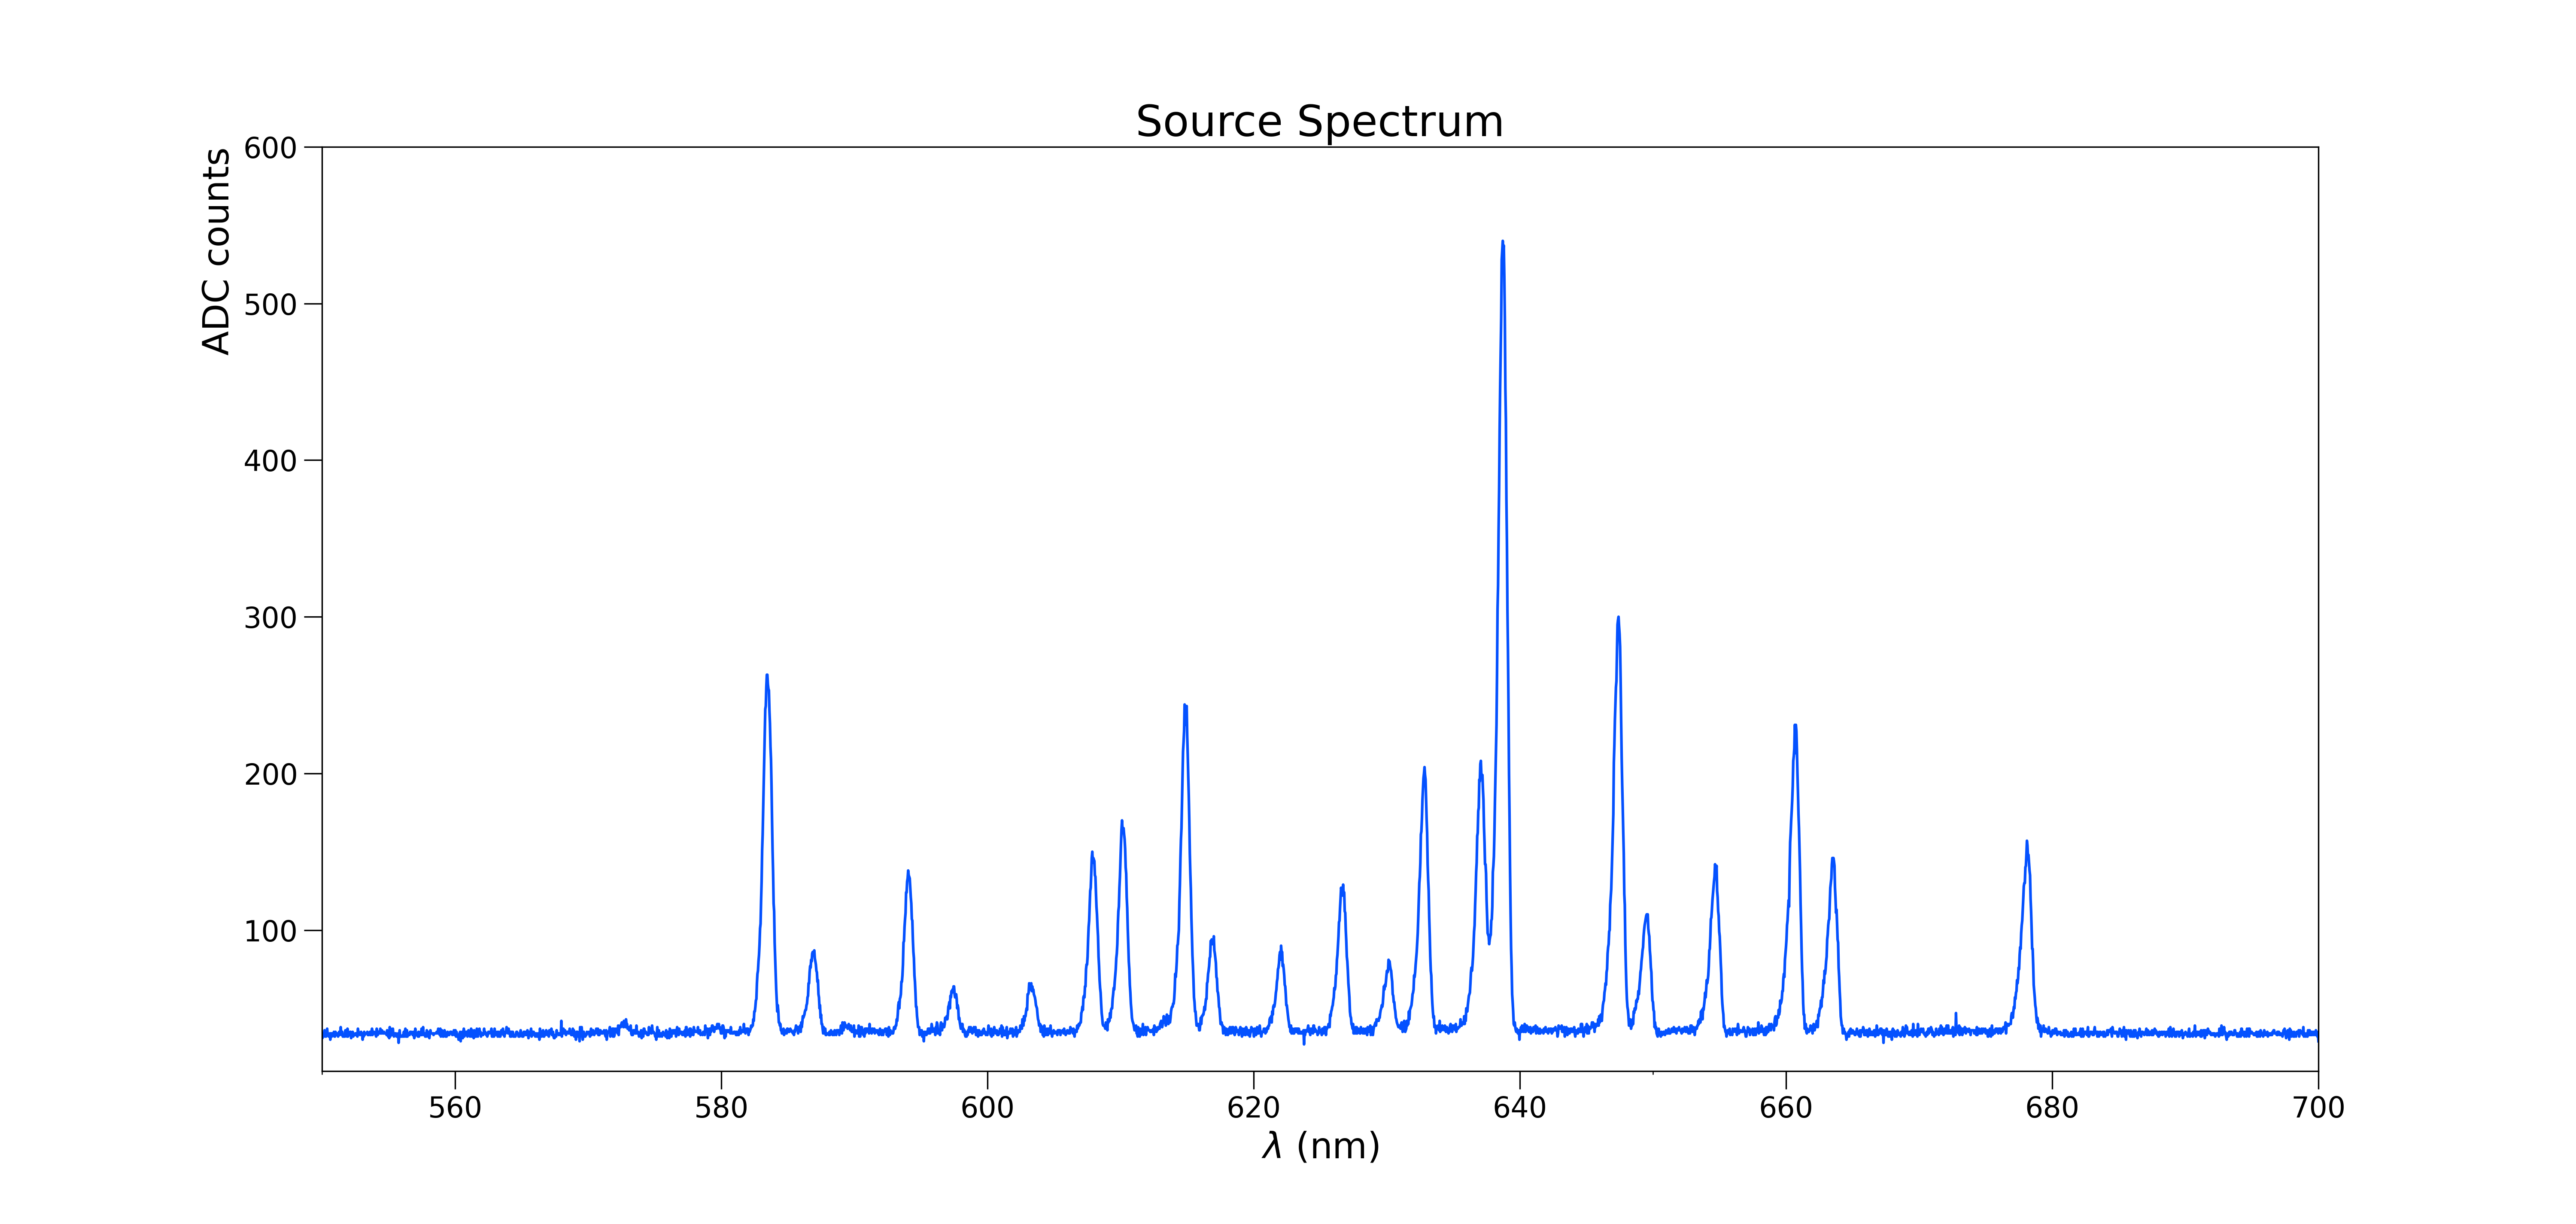
\includegraphics[width=\textwidth]{../Spectrum/SpectrumPlots/spettro1d_Boff.png}
    \caption{Spettro del Neon}
    \label{i:spettro1d}
\end{figure*}


In \figurename\ref{i:spettro1d} si osservano le transizioni nella regione 580-700 \si{\nano \metre}, in particolare la riga più intensa 
a 640.2 \si{\nano \metre} e quella di interesse a 585.3 \si{\nano \metre}.\\
In presenza del campo magnetico, lo spettro rimane invariato, a meno dell'intensità della radiazione che aumenta significativamente. 

% %%%%%%%%%%%%%%%%%%%%%%%%%%%%%%%%%%%%%%%%%%%%%%%%%%%%%%%%%%%%%%%%%%%%%%
\section{Potere risolvente dell'apparato}

\begin{itemize}
    \item Lo calcoliamo con Boff
    \item Formule (range utile ecc ecc) (approx luce radente) 
    \item Procedura di analisi (indipendenza statistica, picchi a triplette ecc ecc)
    \item Plot con tutti i picchi fittati + finestrella con lo zoom su una tripletta
    \item Stima di R (come quando perchè)
    \item Plot del trend per aberrazione 
\end{itemize}
A campo magnetico spento si vuole determinare il potere risolvente dell'apparato, pari a:
\begin{equation}
    R = \frac{\lambda}{\Delta \lambda}
\end{equation}
In approssimazione di luce radente vale:
\begin{equation}
    \Delta \lambda_{\text{r.u.}} \simeq \frac{\lambda^2}{2\text{d}}
    \label{e:lambdaru}
\end{equation}


\begin{figure}
    \centering
    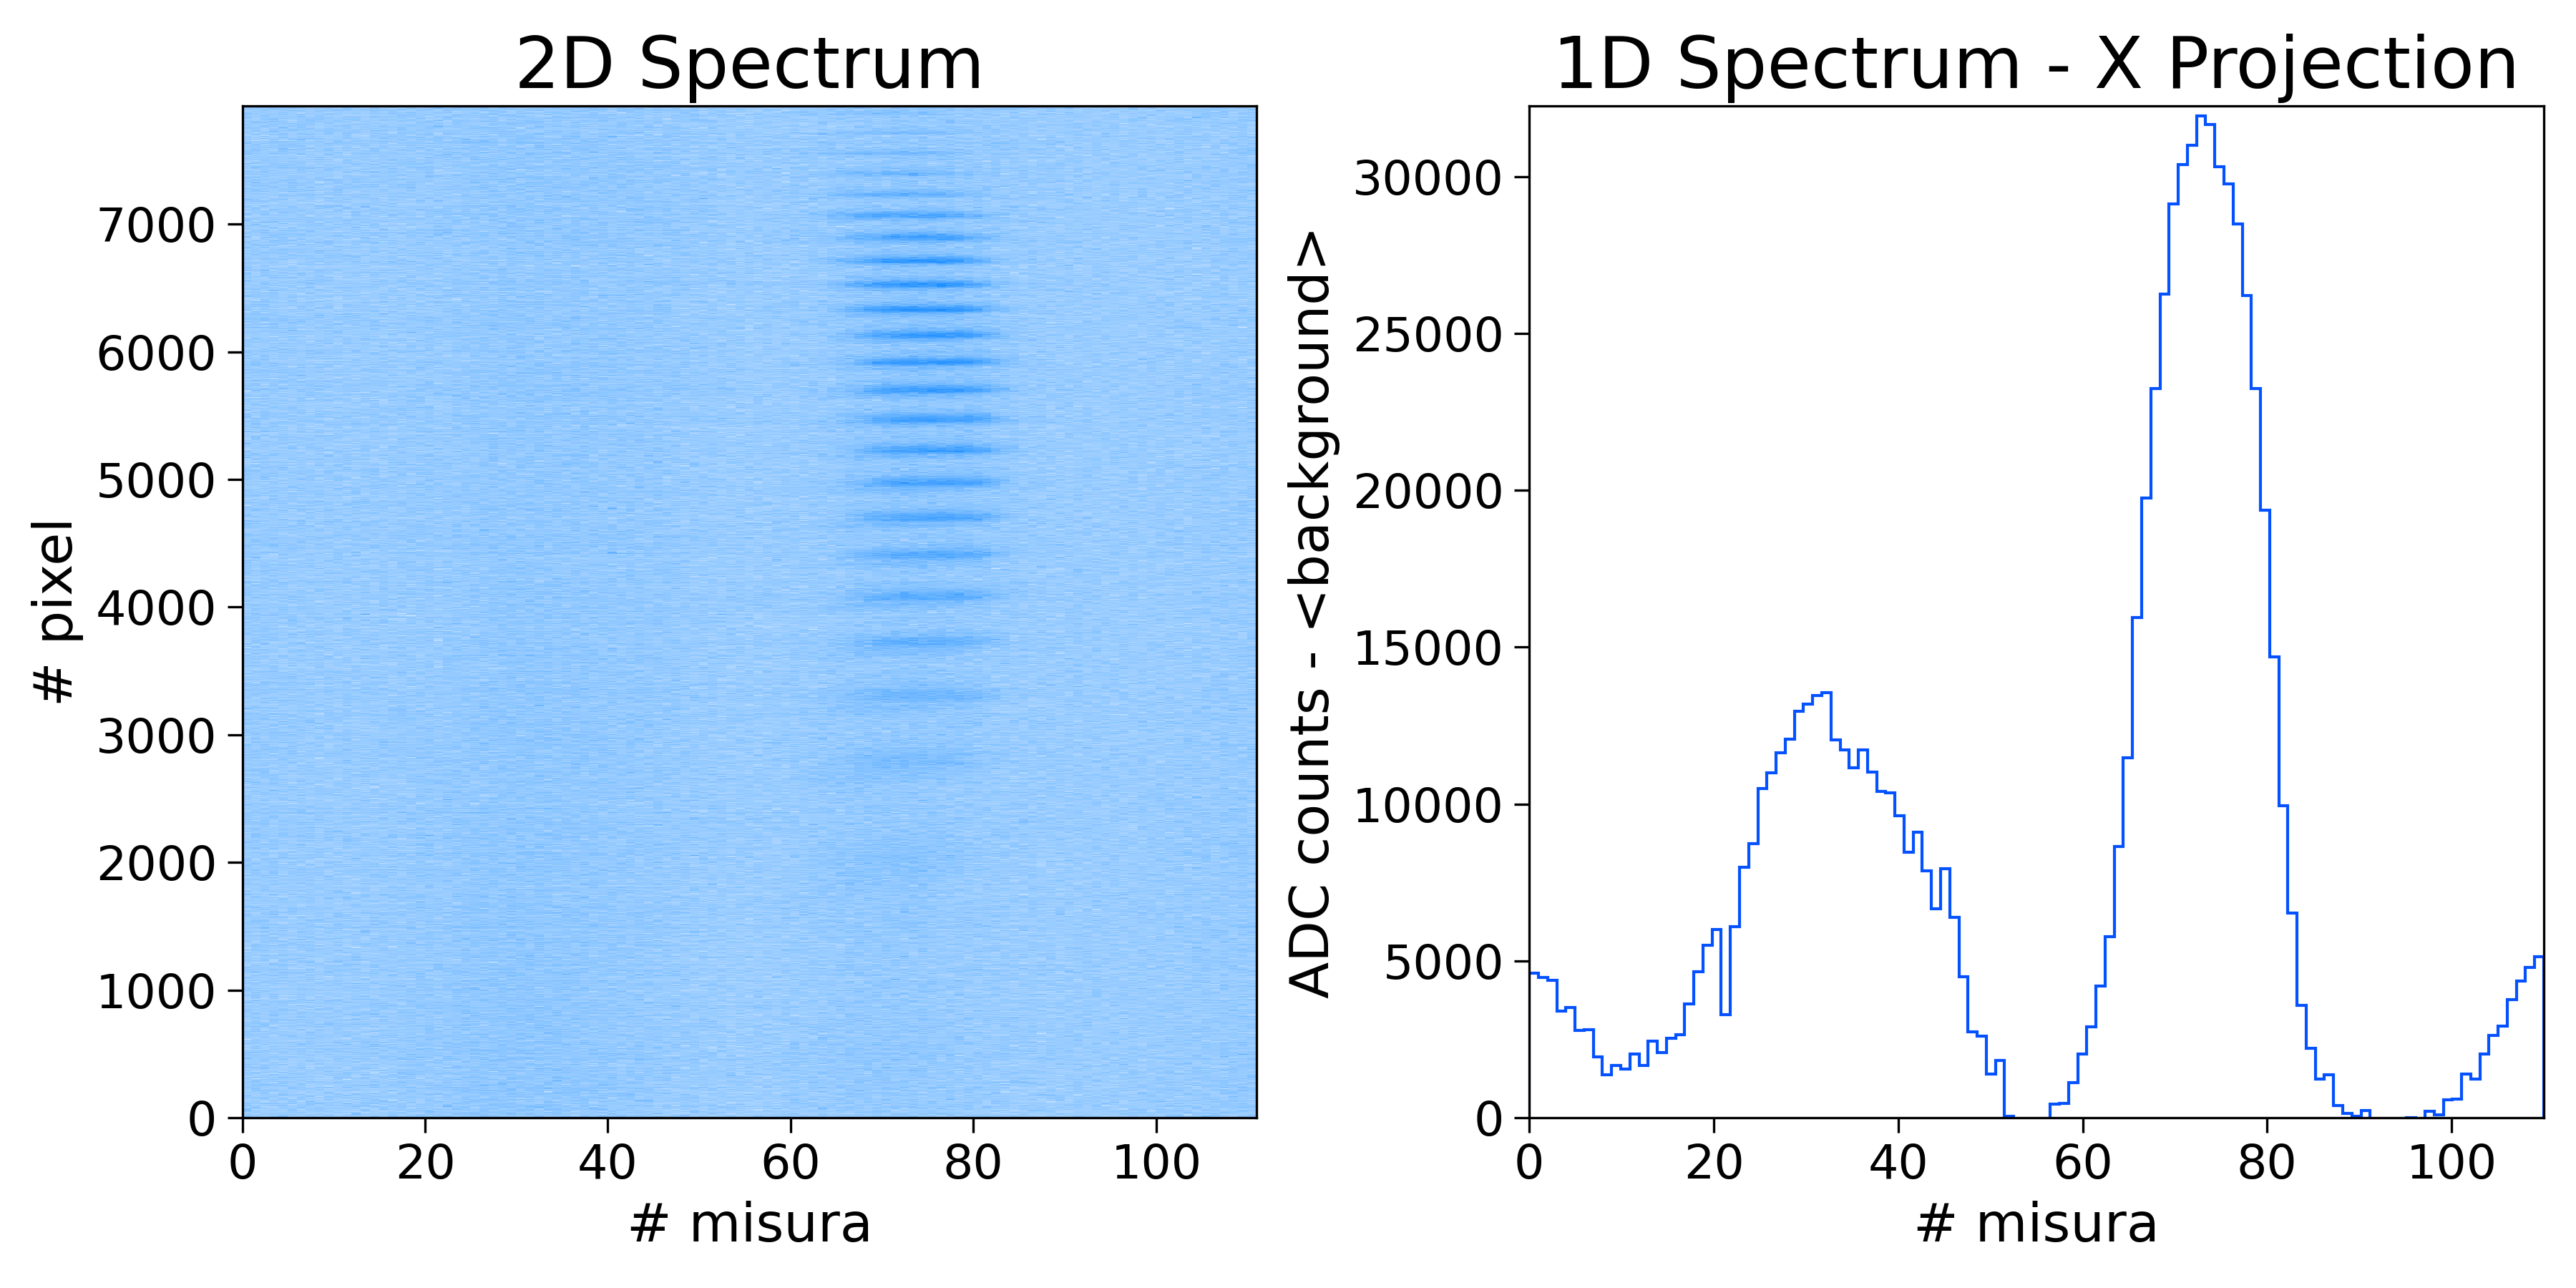
\includegraphics[width=\linewidth]{../Plots/Boff_2d_spectrum.png}
    \caption{Spettro bidimensionale $\text{B}_{off}$}
    \label{i:spettro2d_Boff}
\end{figure}


\begin{figure}
    \centering
    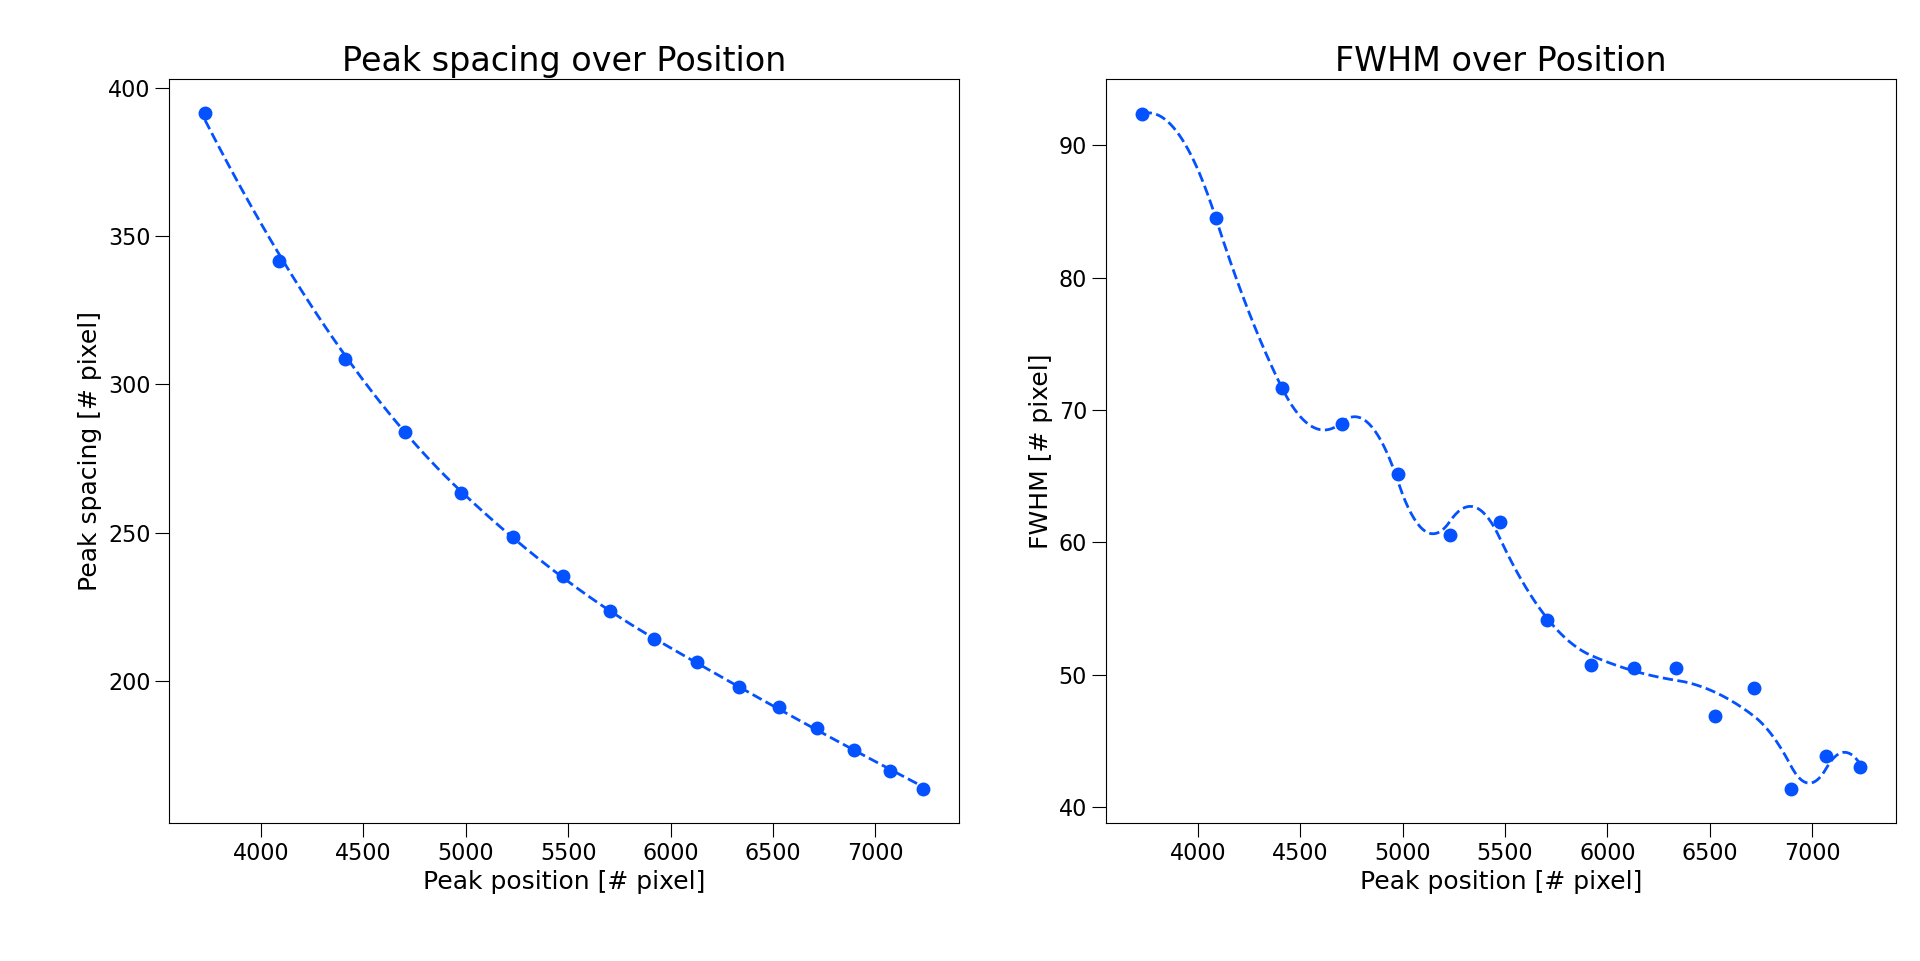
\includegraphics[width=\linewidth]{../Plots/Boff_spacing_trend.png}
    \caption{Spacing trend}
    \label{i:spacing_trend_Boff}
\end{figure}


\begin{figure*}
    \centering
    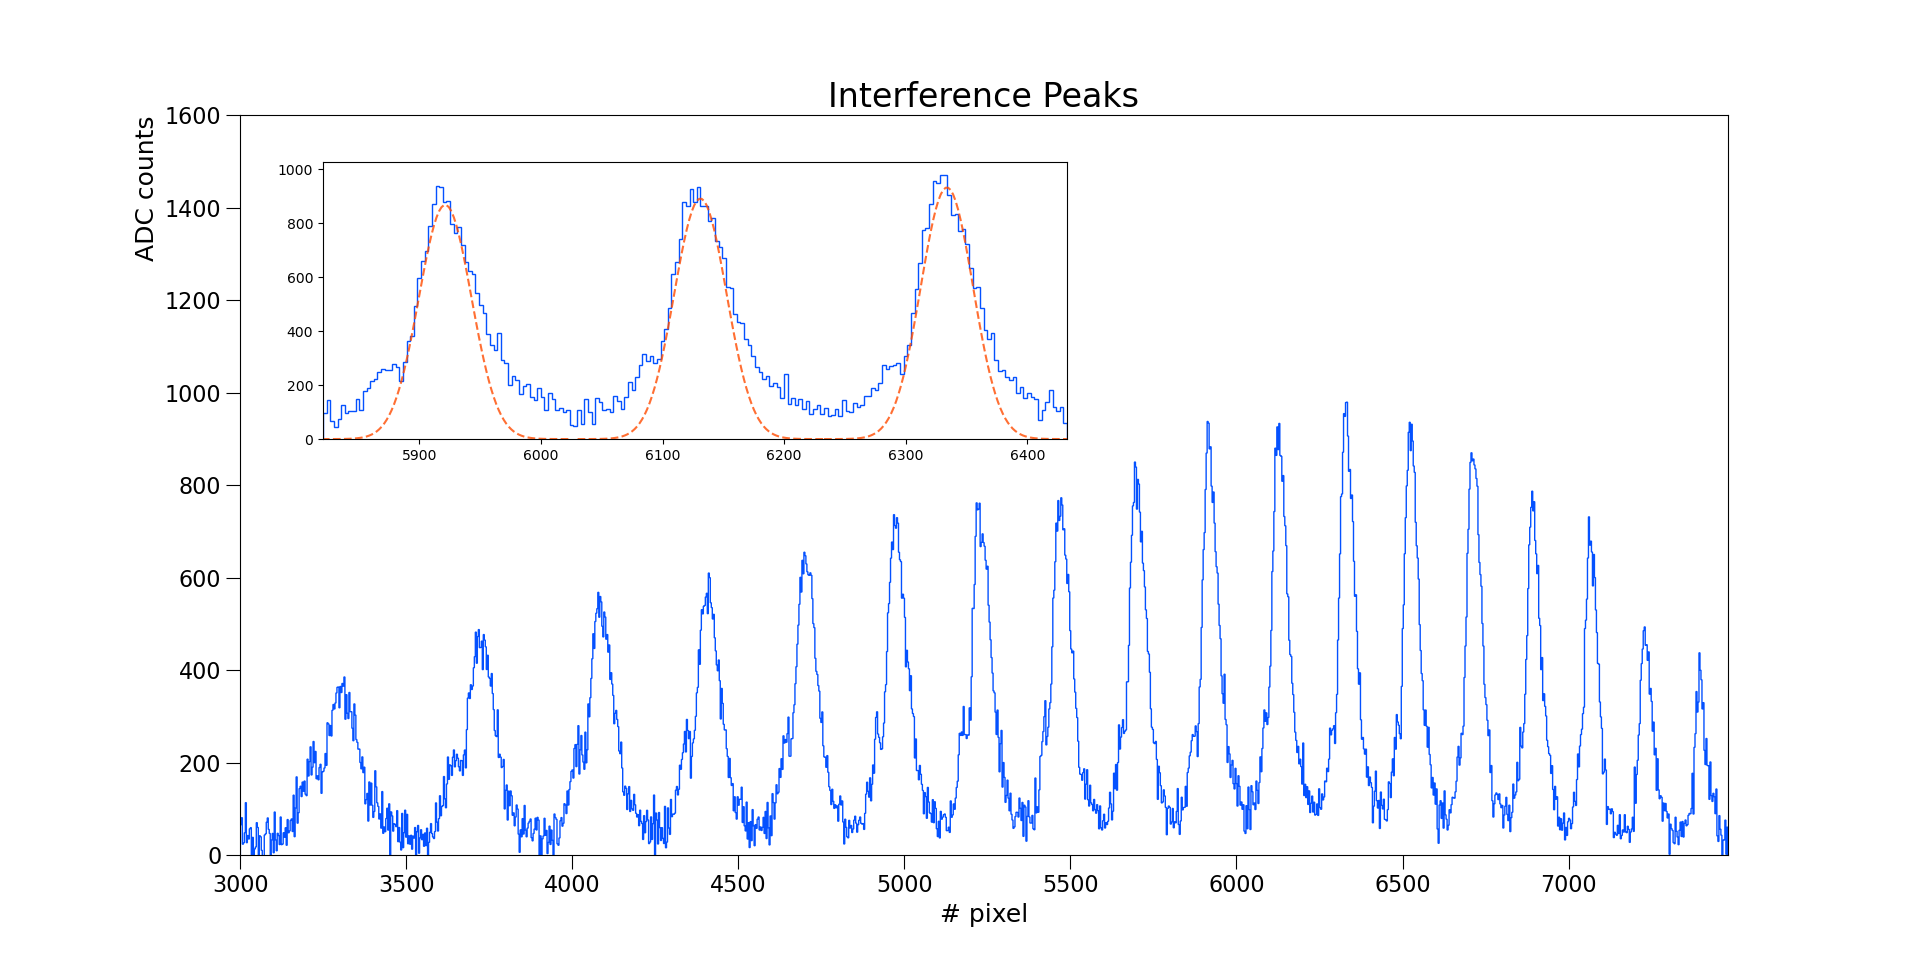
\includegraphics[width=\textwidth]{../Plots/Boff_Y_proj.png}
    \caption{Proiezione sull'asse y $\text{B}_{off}$}
    \label{i:spettro2d_Boff_ProjY}
\end{figure*}





% %%%%%%%%%%%%%%%%%%%%%%%%%%%%%%%%%%%%%%%%%%%%%%%%%%%%%%%%%%%%%%%%%%%%%%
\section{Fattore di Landè}

\begin{itemize}
    \item Lo calcoliamo con Bon lungo la direzione della radiazione (parlare dello splitting di Zeeman)
    \item Formule (range utile + conversione energia + fattore di Landè)
    \item Procedura di analisi (niente fit perchè non vengono)
    \item Plot con tutti i picchi + finestrella con lo zoom su una tripletta 
    \item Controllare che lo splitting Zeeman non subisca aberrazione pesante
\end{itemize}
In questa sezione si analizzano i dati con il campo magnetico acceso e osservando la radiazione parallelamente a $\vec{\text{B}}$.
Poiché un dipolo non emette lungo la direzione che individua, i termini polarizzati circolarmente corrispondenti a $\Delta \text{m} = \pm 1$
hanno intensità maggiore dei termini corrispondenti a $\Delta \text{m} = 0$. Perciò la transizione centrale è soppressa e si osservano solo le due laterali,
separate da $\delta\lambda = 2 \Delta\lambda_{\text{zee}}$
 


\begin{figure*}
    \centering
    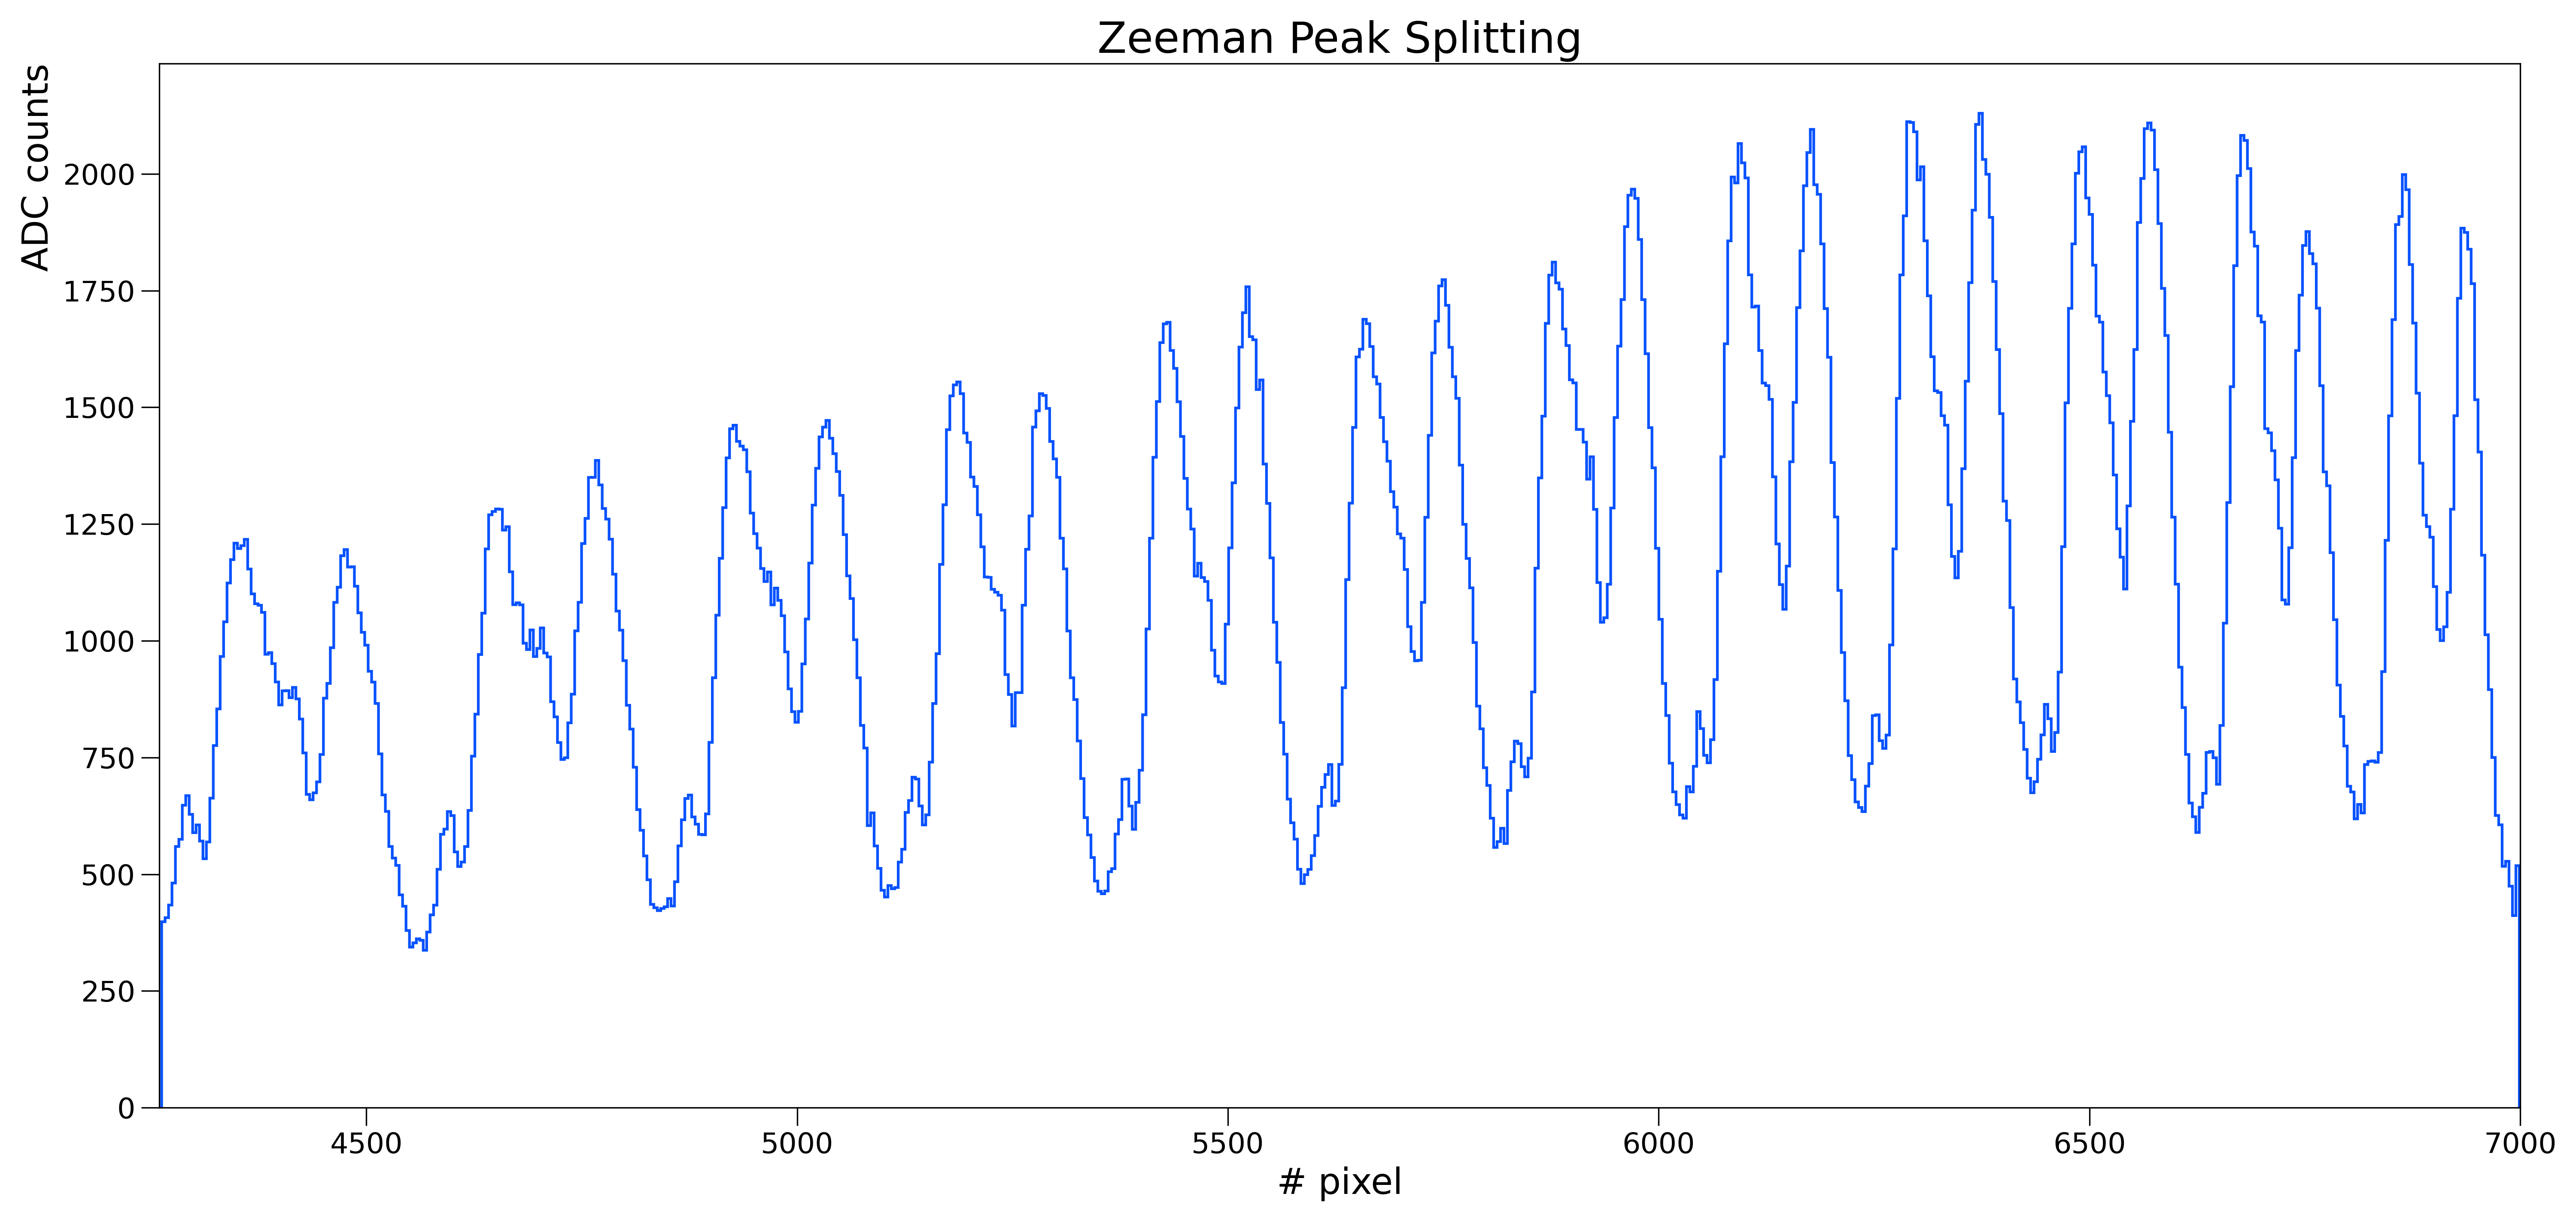
\includegraphics[width=\textwidth]{../Plots/Bon_Y_proj.png}
    \caption{Proiezione sull'asse y $\text{B}_{on}$}
    \label{i:spettro2d_Bon_ProjY}
\end{figure*}

\begin{figure}[h]
    \centering
    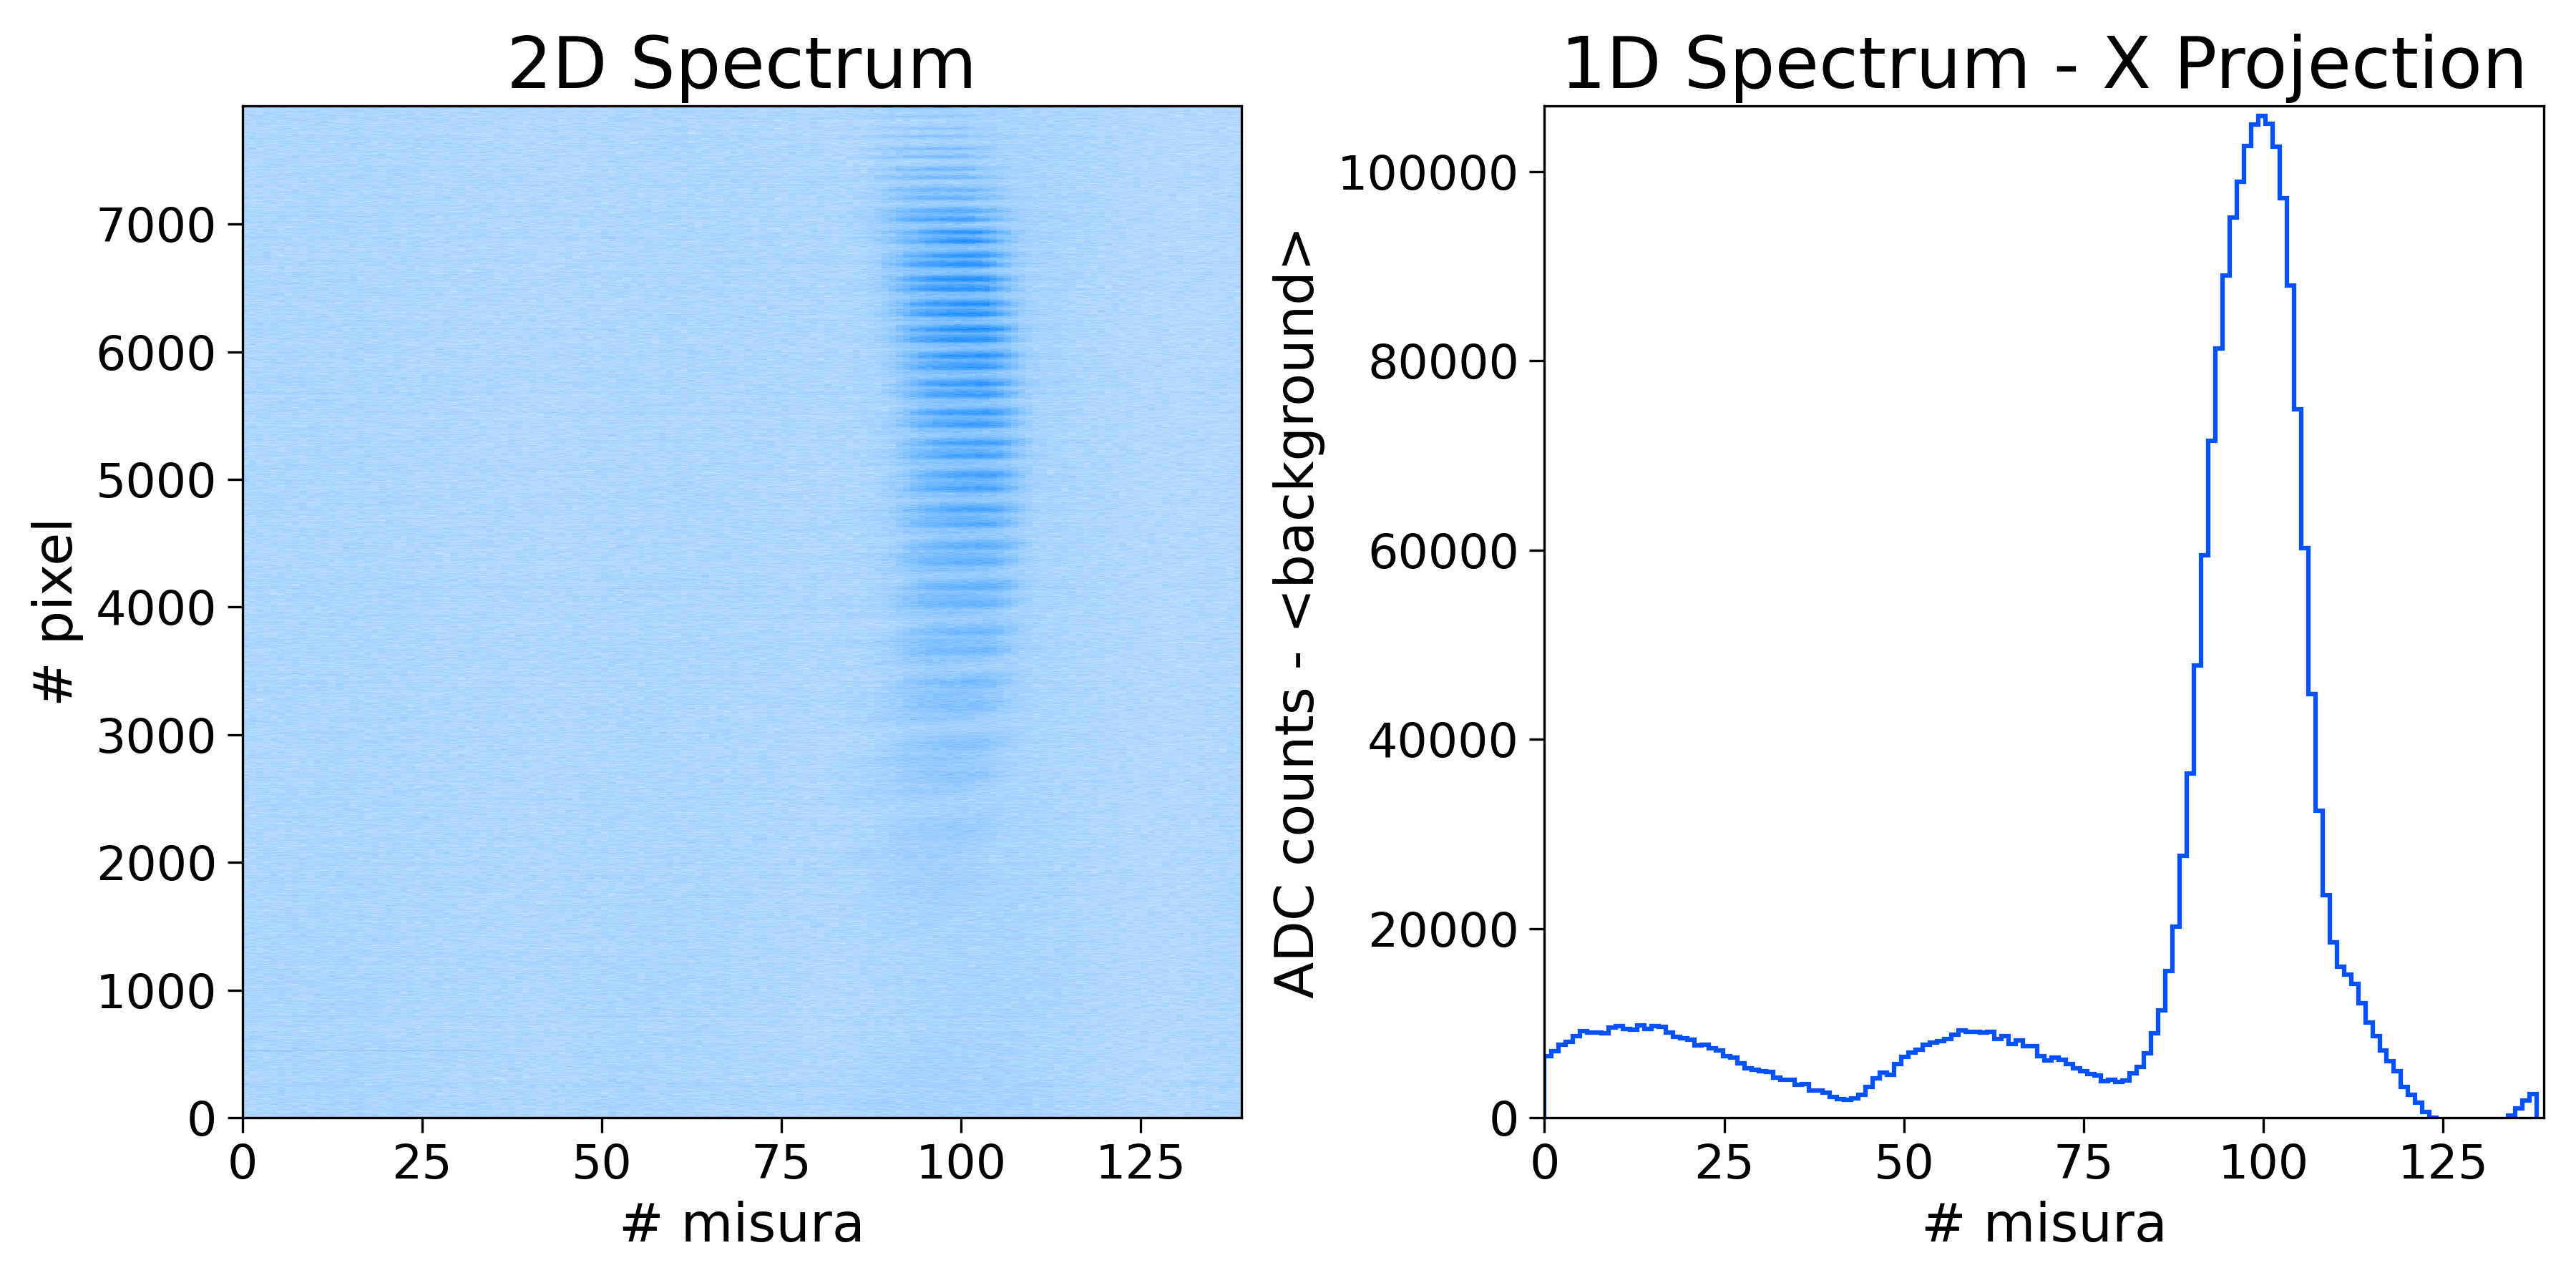
\includegraphics[width=\linewidth]{../Plots/Bon_2d_spectrum.png}
    \caption{Spettro bidimensionale $\text{B}_{on}$}
    \label{i:spettro2d_Bon}
\end{figure}




% %%%%%%%%%%%%%%%%%%%%%%%%%%%%%%%%%%%%%%%%%%%%%%%%%%%%%%%%%%%%%%%%%%%%%%
\section{Campo magnetico ortogonale alla radiazione}

\begin{figure*}
    \centering
    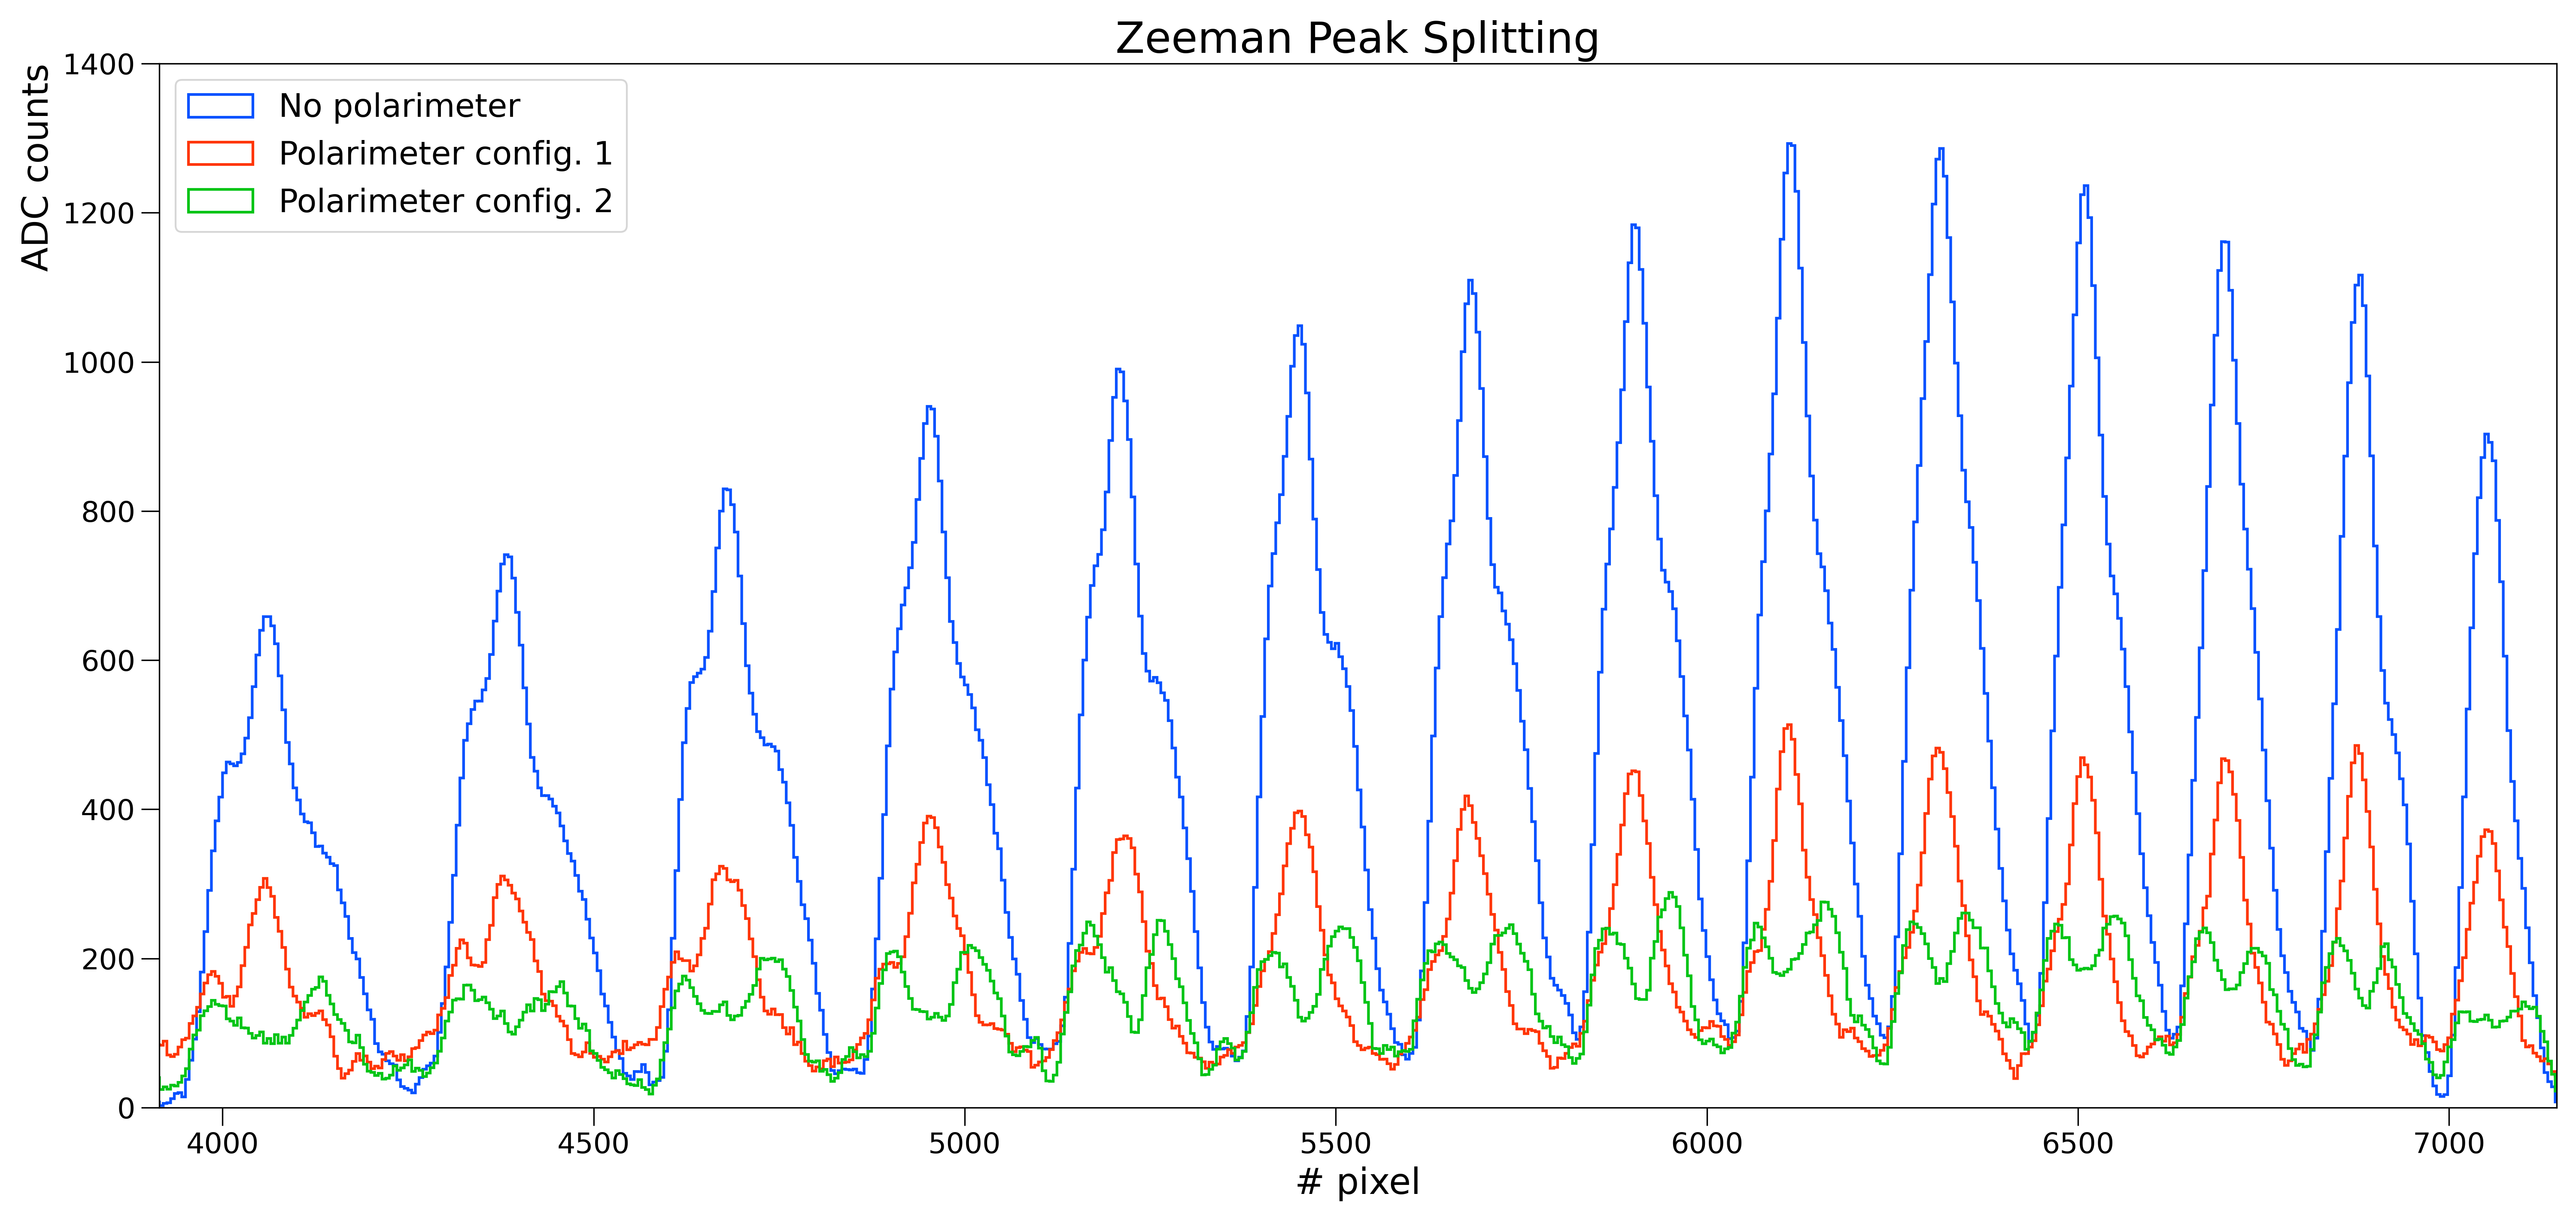
\includegraphics[width=\textwidth]{../Plots/Bon_overlap_big.png}
    \caption{Proiezione sull'asse y dello spettro bidimensionale nelle configurazioni con e senza polarizzatore}
    \label{i:spettro2d_overlap}
\end{figure*}

\begin{itemize}
    \item Un po' di fisica più in dettaglio rispetto all'introduzione (polarizzazione ecc) + aspettative "teoriche"
    (intensità picchi ecc)
    \item Plot istogrammi sovrapposti 
    \item Deduzione configurazioni polarimetro dal plot 
\end{itemize}
Si analizzano i dati acquisiti ruotando il campo magnetico, cioè osservando la radiazione emessa 
in direzione ortogonale a $\vec{\text{B}}$. In questo caso, i termini associati a $\Delta \text{m} = 0$ presentano polarizzazione lineare, 
mentre quelli relativi a $\Delta \text{m} = \pm 1$ sono polarizzati circolarmente in senso orario o antiorario. 
Ci si aspetta quindi di osservare un tripletto, cioè la formazione di tre righe equispaziate visibili nella direzione 
di propagazione trasversa al campo. Successivamente, si inserisce un filtro polarizzatore di fronte alla lente condensante, che viene impiegato in due configurazioni, non note a priori. 
Se il polarizzatore fa passare prevalentemente la componente della luce polarizzata parallelamente alla direzione del campo, allora si osserva una sola riga; se invece, ruotando il filtro, questo 
fa passare la componente della luce con polarizzazione ortogonale al campo, allora la transizione centrale viene soppressa e si osservano solamente i due picchi laterali.
Conseguentemente ci si aspetta che l'intensità della radiazione sia significativamente ridotta con l'inserimento del filtro polarizzatore.  
In \figurename\ref{i:spettro2d_overlap} è riportata la proiezione sull'asse y dello spettro bidimensionale, nelle tre configurazioni precedentamente descritte. 
Si nota che, in generale, l'apparato non permette di risolvere sufficientemente bene le transizioni: questo è particolarmente evidente in assenza del filtro, in quanto
non è possibile distinguere i tre picchi di interferenza distinti che ci si aspetterebbe. Inoltre, si osserva che nella prima configurazione lo spettro è caratterizzato dalla presenza di un unico
picco, mentre nella seconda da un doppietto: da ciò si deduce che nel primo caso il polarizzatore è posto lungo la direzione del campo, mentre nella seconda è ruotato di 90 gradi. 

\end{document}
